\documentclass[11pt]{article}

\usepackage[margin=1in]{geometry}
\usepackage{amsmath,amssymb}
\usepackage{booktabs}
\usepackage{graphicx}
\usepackage{xcolor}
\usepackage{hyperref}
\usepackage{caption}
\usepackage{enumitem}
\usepackage{listings}
\usepackage{float}
\usepackage{fancyhdr}
\usepackage{titlesec}

\hypersetup{
    colorlinks=true,
    linkcolor=blue!50!black,
    citecolor=blue!50!black,
    urlcolor=blue!50!black
}

\lstset{
    basicstyle=\ttfamily\footnotesize,
    breaklines=true,
    columns=fullflexible,
    frame=single,
    backgroundcolor=\color{gray!8},
    xleftmargin=0.5em,
    xrightmargin=0.5em
}

\pagestyle{fancy}
\fancyhf{}
\setlength{\headheight}{14pt}
\fancyhead[L]{Semantic Duplicate \& Near-Plagiarism Detection Engine}
\fancyhead[R]{\thepage}
\renewcommand{\headrulewidth}{0.4pt}

\title{\textbf{Semantic Duplicate \& Near-Plagiarism Detection Engine}\\[0.3em]
\large A Comparative Implementation of Shingling+MinHash+LSH and TF-IDF Weighted SimHash}
\author{Semantic Plagiarism Engine Project}
\date{\today}

\begin{document}

\maketitle

\begin{abstract}
This report documents the design, implementation, and evaluation of an educational, industry-inspired
system for detecting duplicate, copied, and paraphrased documents. Two independent similarity-detection
pipelines are implemented entirely from scratch -- \emph{Shingling + MinHash + Locality-Sensitive Hashing
(LSH)} and \emph{TF-IDF weighted SimHash} -- and compared on a small hand-curated document corpus, a
synthetic labeled question-pair dataset, and the real PAN-PC-11 plagiarism corpus (22{,}186 annotated
document pairs). We describe the text preprocessing pipeline, derive and justify every algorithmic and
hyperparameter choice -- including an automatic threshold-selection procedure that proved necessary once
real, heavily-obfuscated plagiarism cases were evaluated -- report precision/recall/F1 and timing results
across all three datasets, and close with a worked error analysis that highlights the concrete conditions
under which each method succeeds and fails, including a transparently-documented limitation discovered
during the real-corpus evaluation.
\end{abstract}

\tableofcontents

% =========================================================================
\section{Project Overview}
% =========================================================================

Detecting near-duplicate and paraphrased documents is a core subproblem behind plagiarism detection,
news deduplication, search-result clustering, and duplicate-question detection in Q\&A systems. The
central difficulty is that near-duplicates rarely share \emph{identical} text: a plagiarist may reorder
sentences, substitute synonyms, or rewrite passages entirely, while a search engine must still recognize
two differently-worded pages as covering the same content.

This project implements and compares two classical, well-established approaches to this problem:

\begin{enumerate}
    \item \textbf{Shingling + MinHash + LSH}: documents are represented as sets of overlapping word
          $k$-grams (``shingles''); similarity is defined via the Jaccard index over these sets, estimated
          efficiently via MinHash signatures, and candidate pairs are pruned via Locality-Sensitive Hashing
          so that a large corpus never requires exhaustive pairwise comparison.
    \item \textbf{TF-IDF weighted SimHash}: each document is reduced to a single 64-bit fingerprint via a
          weighted, sign-based hash accumulation; similarity is then a simple Hamming-distance computation
          between two fixed-width integers.
    \end{enumerate}

Both pipelines are implemented using only the Python standard library, NumPy, and Pandas -- no
off-the-shelf MinHash/SimHash/LSH library (e.g.\ \verb|datasketch|) is used for the core algorithms. The
project is delivered as a command-line tool (\verb|plagiarism_engine.cli|) with three subcommands
(\verb|compare|, \verb|corpus|, \verb|pairs|); no graphical or terminal UI is provided or required.

% =========================================================================
\section{Text Preprocessing Pipeline}
% =========================================================================

Every document passes through a shared preprocessing pipeline (\verb|preprocessing.py|) before either
detection backend sees it:

\begin{enumerate}[label=\arabic*.]
    \item \textbf{Character normalization}: Unicode NFKC normalization, followed by folding of
          Arabic-script look-alike characters to their canonical Persian forms (e.g.\ ARABIC YEH
          $\rightarrow$ PERSIAN YEH, ARABIC KAF $\rightarrow$ PERSIAN KEHEH) and removal of Arabic
          diacritics (\emph{harakat}), since the specification requires correct handling of Persian text
          in addition to English.
    \item \textbf{Punctuation removal}: both standard ASCII punctuation and common Persian/Arabic
          punctuation marks (the Arabic comma, semicolon and question mark, the percent sign, guillemets,
          the ellipsis character, and the kashida/tatweel elongation character) are stripped.
    \item \textbf{Whitespace collapsing}: consecutive whitespace (including tabs and newlines) is collapsed
          to single spaces.
    \item \textbf{Stop word removal}: a small, explicit stop word list covering both English (\emph{and},
          \emph{is}, \emph{the}, \emph{or}, \ldots) and their Persian equivalents (\emph{va} ``and'',
          \emph{ast} ``is'', \emph{r\={a}} (object marker), \emph{y\={a}} ``or'', \ldots, romanized here for
          typesetting; the actual stop word list in \verb|preprocessing.py| uses native Persian script) is
          removed, exactly as required by the specification.
    \item \textbf{Tokenization}: whitespace tokenization on the normalized text.
    \item \textbf{Shingle construction}: contiguous word $k$-grams are built from the token sequence.
\end{enumerate}

\subsection{Edge case handling}

The specification explicitly calls out three edge cases, all of which are exercised by dedicated
documents in \verb|data/sample_corpus/| and by unit tests in \verb|tests/test_engine.py|:

\begin{itemize}
    \item \textbf{Empty documents} (\verb|doc_09.txt|): produce an empty token list and an empty shingle
          set rather than raising an exception. By convention, two empty documents are treated as
          identical ($J = 1.0$), matching the standard convention for the degenerate $0/0$ Jaccard case.
    \item \textbf{Very short documents} (\verb|doc_07.txt|, five words): if a document has fewer tokens
          than the configured shingle size $k$, the \emph{entire} token sequence is used as a single
          shingle rather than silently producing zero shingles, so short documents remain comparable.
    \item \textbf{Unusual characters} (\verb|doc_08.txt|: emoji, accented Latin letters, em dashes,
          curly quotes): all Unicode control/format/surrogate characters are stripped (while carefully
          preserving whitespace characters, which are technically in the same Unicode general category),
          preventing malformed input from crashing the pipeline or corrupting shingle boundaries.
\end{itemize}

% =========================================================================
\section{Method 1: Shingling + MinHash + LSH}
% =========================================================================

\subsection{Exact Jaccard similarity and its cost}

Given two shingle sets $A$ and $B$, the Jaccard similarity is
\[
    J(A, B) = \frac{|A \cap B|}{|A \cup B|}.
\]
This is implemented directly in \verb|cli.py| (\verb|_exact_jaccard|) and used both as a ground-truth
signal for verification and as the metric MinHash is designed to approximate.

\paragraph{Why exact pairwise comparison is $O(n^2)$.} For a corpus of $n$ documents, finding \emph{all}
pairs whose similarity exceeds some threshold naively requires computing $J(A,B)$ for every unordered pair,
of which there are $\binom{n}{2} = \frac{n(n-1)}{2}$. Each individual Jaccard computation itself costs
$O(|A| + |B|)$ using a hash-set intersection, but the number of \emph{pairs} still grows quadratically in
$n$: doubling the corpus size roughly quadruples the number of comparisons required. For our 11-document
sample corpus this is a trivial 55 comparisons, but for a realistic plagiarism-detection deployment
scanning, say, $n = 100{,}000$ documents, exhaustive comparison would require on the order of $5 \times
10^9$ pairwise set comparisons -- computationally infeasible to run repeatedly. This is precisely the
scaling problem that MinHash + LSH is designed to sidestep.

\subsection{MinHash, implemented from scratch}

MinHash (Broder, 1997) exploits a simple probabilistic fact: for a uniformly random hash function $h$
drawn from a suitable family,
\[
    \Pr\big[\min_{x \in A} h(x) = \min_{x \in B} h(x)\big] = J(A, B).
\]
Drawing $\text{num\_perm}$ independent hash functions and recording, for each one, the minimum hash value
over a document's shingle set produces a fixed-length \emph{signature}. The fraction of signature
positions at which two documents' signatures agree is then an unbiased estimator of their true Jaccard
similarity, with standard error shrinking as $O(1/\sqrt{\text{num\_perm}})$.

\paragraph{Implementation.} \verb|minhash.py| implements the standard universal-hashing family
\[
    h_i(x) = (a_i \cdot x + b_i) \bmod p, \qquad p = 2^{61} - 1 \ \text{(a Mersenne prime)},
\]
with $(a_i, b_i)$ drawn once per \verb|MinHasher| instance from a seeded random generator. Because
Python's built-in \verb|hash()| is randomized per-process (for security reasons, via
\verb|PYTHONHASHSEED|), it cannot be used to map shingle strings to integers -- the same shingle must hash
identically across every document and every run for MinHash to work at all. We instead use SHA-1
(truncated to 64 bits) as a stable base hash (\verb|stable_hash|), and apply the universal hash family on
top of that integer.

An empty shingle set produces a sentinel all-maximum-value signature; two empty documents therefore compare
as identical, consistent with the Jaccard convention above.

\subsection{LSH (banding), implemented from scratch}

A MinHash signature of length \verb|num_perm| is split into \verb|num_bands| contiguous bands of
$r = \text{num\_perm} / \text{num\_bands}$ rows each. Each band is hashed (SHA-1 over the band's raw
signature values, salted with the band index so that identical row values in different bands never
collide with each other) to a bucket key. Two documents become \emph{candidates} for further comparison
if and only if at least one of their bands maps to the same bucket.

\paragraph{Why this reduces comparisons.} Only documents that collide in a bucket are ever compared with
exact Jaccard; documents that share no band never enter the candidate set at all. Section~\ref{sec:results}
reports the actual reduction achieved on the sample corpus (94.55\%, i.e.\ only 3 of 55 possible pairs were
ever verified).

\paragraph{The S-curve and parameter selection.} The banding scheme induces a well-known ``S-curve''
relationship between a pair's true Jaccard similarity $s$ and its probability of becoming a candidate:
\[
    P(\text{candidate} \mid s) = 1 - (1 - s^r)^b,
\]
implemented as \verb|candidate_probability| in \verb|lsh.py|. This function is close to $0$ for $s$ below
a threshold and close to $1$ above it, with the steepest transition near
\[
    s^{*} = \Big(\frac{1}{b}\Big)^{1/r}
\]
(\verb|s_curve_threshold|). Figure~\ref{fig:s-curve} plots this curve for three different
(\verb|num_bands|, \verb|rows_per_band|) splits of a 128-permutation signature. Fewer, larger bands
(e.g.\ $b=8, r=16$) push the transition threshold higher (fewer false-positive candidates, but a steeper,
less forgiving curve that misses moderately-similar pairs); more, smaller bands (e.g.\ $b=32, r=4$) push
the threshold lower (catches weaker similarity, at the cost of generating more candidate pairs that need
exact verification). This is a direct, tunable trade-off between recall (of the candidate-generation step)
and computational cost of the verification step.

\begin{figure}[H]
    \centering
    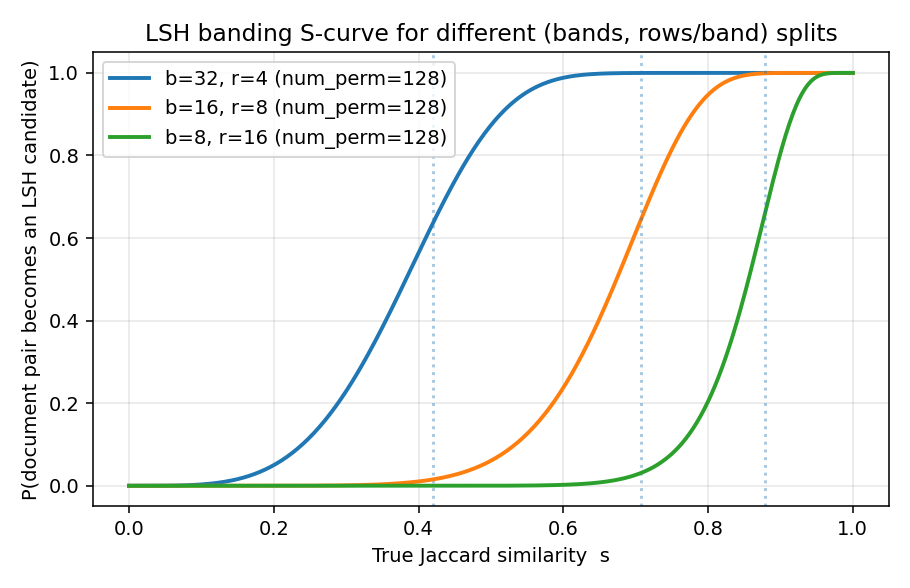
\includegraphics[width=0.72\textwidth]{figures/lsh_s_curve.png}
    \caption{LSH banding S-curve for three (bands, rows-per-band) configurations of a 128-permutation
    MinHash signature. Dotted vertical lines mark each configuration's approximate detection threshold
    $s^{*} = (1/b)^{1/r}$.}
    \label{fig:s-curve}
\end{figure}

% =========================================================================
\section{Method 2: TF-IDF Weighted SimHash}
% =========================================================================

SimHash (Charikar, 2002) takes a different approach: rather than representing a document as a \emph{set},
it accumulates a single fixed-width fingerprint such that similar documents land at small Hamming
distance from one another, turning similarity search into simple bit-counting.

\paragraph{Algorithm.} For a document represented as a weighted bag of tokens $\{(\text{term}, w)\}$:
\begin{enumerate}[label=\arabic*.]
    \item Initialize a 64-dimensional accumulator $V = \mathbf{0}$.
    \item For each term, compute a stable 64-bit hash of the term (BLAKE2b, again avoiding Python's
          randomized built-in \verb|hash()|).
    \item For each of the 64 bit positions $i$: if bit $i$ of the term's hash is $1$, add the term's
          weight $w$ to $V_i$; otherwise subtract $w$ from $V_i$.
    \item The final fingerprint bit $i$ is $1$ if $V_i > 0$, else $0$.
\end{enumerate}
The weight $w$ of each term is its TF-IDF score, computed from scratch in \verb|TfidfVectorizerFromScratch|
using the standard smoothed formulation
\[
    \text{idf}(t) = \ln\!\left(\frac{1+N}{1+\text{df}(t)}\right) + 1,
\]
so that a term appearing in \emph{every} document of the fitted corpus still receives a small positive
weight rather than exactly zero, and unseen terms at inference time fall back sensibly to the corpus's
maximum IDF. Similarity between two fingerprints is reported both as raw Hamming distance
(\verb|hamming_distance|) and as a normalized similarity in $[0,1]$
(\verb|hamming_similarity| $= 1 - d_H / 64$).

\paragraph{Why TF-IDF weighting matters.} An unweighted SimHash (equal weight per token) would let common,
low-information words dominate the fingerprint. Weighting each term's contribution by its corpus-level rarity
concentrates the fingerprint's discriminative power on the words that actually distinguish one document's
topic from another's -- the SimHash analogue of stop-word removal, but continuous rather than binary.

% =========================================================================
\section{Parameter Selection}
\label{sec:params}
% =========================================================================

\subsection{Shingle size ($k$)}
\label{sec:shingle-size-short}

The specification recommends $k \in \{3, 4, 5\}$ for shingling. This recommendation implicitly assumes
paragraph-length documents; for the paragraph-length demo documents in \verb|data/sample_corpus/|
(50--75 tokens each), $k=3$ produces shingle sets large enough (50--70 shingles per document) to give
MinHash a stable signal while still being sensitive to word-level edits.

Short, sentence-length text behaves very differently. Table~\ref{tab:threshold-sweep} shows a threshold
sweep of the best achievable F1 score at different shingle sizes on the synthetic question-pair dataset
(Section~\ref{sec:pairs-dataset}), where each document is a single $\sim$10-word question: $k=3$ shingles
leave only 6--9 shingles per document, so a single word substitution can eliminate the majority of a
document's shingles outright, collapsing the Jaccard signal. Reducing $k$ to $1$ (i.e.\ plain word-overlap
Jaccard) recovers substantially more signal for short documents. \textbf{We therefore use $k=3$ as the
default for the \texttt{compare}/\texttt{corpus} commands (paragraph-length documents) and $k=1$ for the
\texttt{pairs} demo run against the short, question-length dataset}, and expose \verb|--shingle-size| as a
CLI flag so it can be tuned to the target corpus's typical document length.

\begin{table}[H]
    \centering
    \caption{Best achievable F1 (via threshold sweep) on the synthetic question-pair dataset, by shingle
    size / method. Lower shingle sizes recover more signal for short, sentence-length documents.}
    \label{tab:threshold-sweep}
    \begin{tabular}{@{}llrrr@{}}
        \toprule
        Method & Config & Best threshold & Precision & Recall / F1 \\
        \midrule
        MinHash+LSH & $k=1$ & $0.13$ & $0.730$ & $0.900\ /\ 0.806$ \\
        MinHash+LSH & $k=2$ & $0.01$ & $0.697$ & $0.767\ /\ 0.730$ \\
        MinHash+LSH & $k=3$ & $0.01$ & $0.783$ & $0.600\ /\ 0.679$ \\
        TF-IDF SimHash & 64-bit & $0.46$ & $0.556$ & $1.000\ /\ 0.714$ \\
        \bottomrule
    \end{tabular}
\end{table}

\subsection{MinHash signature length (\texttt{num\_perm})}

The specification recommends 128 or 256 permutations. The estimation standard error of the MinHash Jaccard
estimate is approximately $1/\sqrt{\text{num\_perm}}$: about $8.8\%$ at 128 permutations, and about
$6.25\%$ at 256. We use \textbf{128} as the default, which is a reasonable balance of accuracy against
signature-computation cost (each additional permutation is one more $O(|\text{shingles}|)$ min-scan per
document) for a project of this scale; \verb|--num-perm| is exposed for anyone who wants the higher
accuracy of 256 at double the cost.

\subsection{LSH bands (\texttt{num\_bands})}

With $\text{num\_perm}=128$, we default to $\text{num\_bands}=32$ (so $r=4$ rows per band), giving an
approximate detection threshold of $s^{*} = (1/32)^{1/4} \approx 0.42$ (Figure~\ref{fig:s-curve}). This
was chosen empirically to be low enough to reliably surface the ``light near-duplicate'' case in the demo
corpus (\verb|doc_01.txt| vs.\ \verb|doc_11.txt|, true Jaccard $\approx 0.48$) as an LSH candidate, while
still being high enough that completely unrelated documents essentially never collide by chance.

\subsection{SimHash bit width}

Fixed at 64 bits per the specification. 64 bits is also the machine word size on essentially all modern
hardware, which keeps Hamming-distance computation (\verb|bin(a ^ b).count("1")|) cheap.

\subsection{Decision thresholds}

Every CLI command's similarity threshold is exposed as a flag rather than hard-coded
(\verb|--threshold| for \texttt{corpus}, \verb|--minhash-threshold| / \verb|--simhash-threshold| for
\texttt{pairs}), because, as Table~\ref{tab:threshold-sweep} demonstrates, the right operating point
depends heavily on document length and on the relative cost of false positives vs.\ false negatives in the
deployment context (e.g.\ a plagiarism screening tool used to flag work for \emph{human} review can
tolerate a lower precision / higher recall operating point than one that takes automated action).

\subsection{Automatic threshold selection (\texttt{--sweep})}
\label{sec:sweep}

Manually guessing a threshold and hoping it transfers to a new dataset turned out, in practice, to be
unreliable enough that it warranted first-class tool support rather than a one-off analysis script. The
\texttt{pairs} command accepts a \verb|--sweep| flag: each pair's similarity score is computed exactly
once (via \verb|compute_minhash_similarities| / \verb|compute_simhash_similarities| in
\verb|evaluation.py|), and then re-thresholded across a grid (default: $0.00$ to $1.00$ in steps of
$0.02$) via \verb|sweep_thresholds|, with the F1-maximizing threshold selected by
\verb|best_threshold_row|. Because scoring dominates the cost and re-thresholding a precomputed score list
is $O(1)$ per threshold, a full sweep costs barely more than a single fixed-threshold run. The chosen
threshold is recorded in the output (\verb|threshold_used| column) so results stay reproducible, and
\verb|--sweep-output| can save the entire precision/recall/F1-vs-threshold curve for further analysis
(Figure~\ref{fig:threshold-sweep-curve}).

\begin{figure}[H]
    \centering
    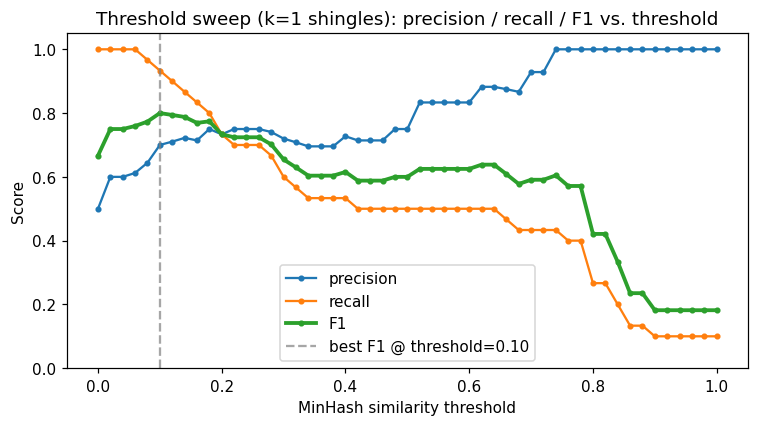
\includegraphics[width=0.72\textwidth]{figures/threshold_sweep_curve.png}
    \caption{Precision, recall, and F1 as a function of the MinHash similarity threshold ($k=1$), swept
    on the synthetic labeled pair dataset. The dashed line marks the F1-maximizing threshold that
    \texttt{--sweep} selects automatically.}
    \label{fig:threshold-sweep-curve}
\end{figure}

This capability was added specifically in response to a real failure mode encountered when evaluating on
PAN-PC-11 (Section~\ref{sec:pan-pc11-results}): the fixed default thresholds tuned for one text regime
produced near-\emph{perfect precision but collapsed recall} on another, a diagnostic pattern worth naming
explicitly since it is easy to mistake for a broken similarity measure rather than a miscalibrated decision
boundary. A sweep resolves this whenever a usable threshold exists at all; Section~\ref{sec:pan-pc11-results}
also documents a case where the sweep reveals that \emph{no} threshold beats the trivial ``always predict
duplicate'' baseline, which is itself diagnostic information about a hyperparameter choice, not a tool
failure.

\subsection{Shingle size revisited: long, obfuscated spans (PAN-PC-11)}
\label{sec:shingle-size-pan}

Section~\ref{sec:shingle-size-short} showed that short questions need a smaller shingle size than the specification's
recommended $k \in \{3,4,5\}$ because there simply isn't enough text to form many shingles. The real
PAN-PC-11 corpus (Section~\ref{sec:pan-pc11-dataset}) motivates the same conclusion, $k=1$, for the
\emph{opposite} reason: its plagiarism spans are long (observed annotated span lengths ranged from 1{,}421
to 18{,}006 characters) but are frequently \emph{obfuscated} by scattering word-level substitutions
throughout the passage rather than rewriting contiguous phrases. A single substituted word destroys every
overlapping $k$-word shingle; over a long span with many scattered substitutions this compounds and can
erase most of the true overlap even though the vast majority of the passage's vocabulary is still shared.
Unigram shingling (effectively plain bag-of-words Jaccard) is largely insensitive to \emph{where} an edit
falls, at the cost of no longer testing local word order at all. Table~\ref{tab:pan-pc11-results} quantifies
the resulting difference: $F_1$ rises from $0.070$ at $k=3$ (fixed thresholds) to $0.920$ at $k=1$ (swept
threshold) for MinHash+LSH on the same 4{,}000-pair evaluation set. \textbf{We therefore treat shingle size
as a corpus-dependent hyperparameter tuned per deployment, not a fixed constant} -- $k=3$ remains the
default for the \texttt{compare}/\texttt{corpus} commands as a paragraph-length-appropriate starting point,
but both real evaluations in this report needed a smaller value once actual data was used.

% =========================================================================
\section{Datasets}
\label{sec:pairs-dataset}
% =========================================================================

\subsection{Recommended large-scale datasets (not bundled)}

Per the specification, large raw datasets are \emph{not} included in this repository. \verb|data/raw/README.md|
documents how to obtain and wire up any of the three recommended datasets:

\begin{itemize}
    \item \textbf{PAN-PC-11} (PAN 2011 Plagiarism Corpus) -- the primary recommended dataset, containing
          both manually and automatically obfuscated plagiarism cases, available via Zenodo.
    \item \textbf{Stack Exchange Duplicates} -- duplicate-marked Q\&A post pairs, available on the
          Hugging Face Hub.
    \item \textbf{Quora Question Pairs} -- 400{,}000+ question pairs labeled duplicate / non-duplicate,
          available on the Hugging Face Hub / Kaggle.
\end{itemize}

\subsection{Sample corpus (\texttt{data/sample\_corpus/})}

An 11-document corpus was hand-authored to exercise every case discussed in this report at once:
one source paragraph on renewable energy (\verb|doc_01.txt|) with a verbatim copy (\verb|doc_03.txt|,
simulated copy-paste plagiarism), a lightly-edited near-duplicate (\verb|doc_11.txt|, minor word
substitutions), and a heavily-paraphrased near-duplicate (\verb|doc_02.txt|, full rewrite); a second,
unrelated source paragraph on Mars exploration (\verb|doc_04.txt|) with its own heavy paraphrase
(\verb|doc_05.txt|); an unrelated cooking paragraph (\verb|doc_06.txt|); and four edge-case documents
(very short, unusual characters, empty, and Persian-language).

\subsection{Synthetic labeled pair dataset (\texttt{data/raw/quora/sample\_pairs.csv})}

Because the build environment used for this report has no network access, the real Quora Question Pairs
dataset could not be downloaded. A 60-row synthetic dataset was hand-authored in the same schema
(\verb|question1, question2, is_duplicate|) to make the \texttt{pairs} command runnable and evaluable out
of the box. It deliberately spans four difficulty tiers, 15 pairs each except where noted:

\begin{itemize}
    \item \textbf{Light duplicates} (15 pairs, label 1): the same question with a minor wording change
          (e.g.\ \emph{``How can I improve my English speaking skills?''} vs.\ \emph{``How can I improve
          my English speaking ability?''}) -- high lexical overlap, the easy case.
    \item \textbf{Heavy duplicates} (15 pairs, label 1): the same question fully reworded with different
          vocabulary (e.g.\ \emph{``What is the difference between machine learning and deep learning?''}
          vs.\ \emph{``How does deep learning differ from machine learning?''}) -- low lexical overlap,
          the hard case for lexical methods.
    \item \textbf{Easy negatives} (24 pairs, label 0): unrelated topics, near-zero expected overlap.
    \item \textbf{Hard negatives} (6 pairs, label 0): the \emph{same sentence template} with one key
          content word swapped (e.g.\ \emph{``How do I learn to play the piano as an adult?''} vs.\
          \emph{``How do I learn to play chess as an adult?''}) -- high lexical overlap despite being
          semantically different questions, deliberately designed to probe the failure mode of purely
          lexical similarity measures.
\end{itemize}

This design intentionally does \emph{not} produce an easy 100\%-accuracy dataset; it is meant to surface
the genuine trade-offs discussed in Section~\ref{sec:error-analysis}, in the same spirit as the real Quora
Question Pairs corpus, which also contains many lexically-similar-but-non-duplicate question pairs.

\subsection{The real PAN-PC-11 corpus}
\label{sec:pan-pc11-dataset}

Beyond the synthetic question-pair dataset above, the primary specified dataset -- the real PAN-PC-11
corpus (Zenodo, DOI 10.5281/zenodo.3250095) -- was downloaded and evaluated directly. Its confirmed
directory layout is:

\begin{lstlisting}
pan-plagiarism-corpus-2011/
    external-detection-corpus/
        source-document/part1/ ... part23/       source-documentKKKKKK.{txt,xml}
        suspicious-document/part1/ ... part23/    suspicious-documentKKKKKK.{txt,xml}
    intrinsic-detection-corpus/
        suspicious-document/part1/ ... part10/    (no source documents; not used here)
\end{lstlisting}

Each suspicious document's XML sibling annotates injected plagiarism cases as a feature element:

\begin{lstlisting}
<feature name="plagiarism" this_offset="..." this_length="..."
         source_reference="..." source_offset="..." source_length="..." />
\end{lstlisting}

confirmed directly against the real corpus (not merely assumed from the published schema) via a
purpose-built inspection tool, \verb|scripts/prepare_pan_pc11_pairs.py --inspect|, which enumerates every
distinct \texttt{<feature name="...">} value actually present before any pairs are built.

\paragraph{Building a labeled pair CSV from raw annotations.} The same script converts the annotation
format into the \verb|text_a, text_b, label| schema the \texttt{pairs} command already expects, with no
changes to \verb|src/plagiarism_engine/| required. Under \verb|external-detection-corpus|, it found
22{,}186 matched (\texttt{.txt}, \texttt{.xml}) file pairs (11{,}093 suspicious-document / 11{,}093
source-document). From these, 2{,}000 positive pairs were built by extracting the exact annotated
this-document/source-document span pair for each real \texttt{plagiarism} feature (0 skipped, 0 XML parse
errors), and 2{,}000 negative pairs were built by sampling random excerpts from unrelated documents,
explicitly excluding the 864 document pairs that have a genuine plagiarism relationship annotated
\emph{elsewhere} in the corpus (so a negative pair is never accidentally drawn from two documents that are
known to be related) -- 4{,}000 pairs total.

\paragraph{A known limitation of this construction.} Positive-pair spans use the exact annotated length
(\verb|this_length|), which the corpus lets vary enormously (observed range: 1{,}421--18{,}006 characters);
negative pairs, for implementation simplicity, are built from excerpts capped at $\sim$1{,}000 characters.
This creates a systematic length difference between the positive and negative classes that this report
does not claim to have controlled for: sheer text length is itself weakly predictive of the label here, on
top of whatever genuine lexical-overlap signal exists. The qualitative finding in
Section~\ref{sec:shingle-size-pan} (that $k=1$ dramatically outperforms $k=3$ under obfuscation) is
unaffected, since both configurations are evaluated on the identical dataset -- but the absolute precision/
recall/F1 values in Table~\ref{tab:pan-pc11-results} should be read with this caveat rather than as a
fully length-controlled measurement. See Section~\ref{sec:limitations} for a proposed fix.

% =========================================================================
\section{Experimental Evaluation}
\label{sec:results}
% =========================================================================

\subsection{Corpus-level results: comparisons avoided by LSH}
\label{sec:corpus-results}

Running \verb|plagiarism_engine.cli corpus| against the 11-document sample corpus
($\text{shingle\_size}=3$, $\text{threshold}=0.25$, $\text{num\_perm}=128$, $\text{num\_bands}=32$)
produces the following summary:

\begin{table}[H]
    \centering
    \caption{LSH candidate-generation summary on the 11-document sample corpus.}
    \begin{tabular}{@{}lr@{}}
        \toprule
        Documents scanned & 11 \\
        Total possible pairs, $\binom{n}{2}$ & 55 \\
        LSH candidate pairs & 3 \\
        \textbf{Comparisons avoided by LSH} & \textbf{94.55\%} \\
        Pairs above threshold (0.25) after exact verification & 3 \\
        \bottomrule
    \end{tabular}
\end{table}

\begin{figure}[H]
    \centering
    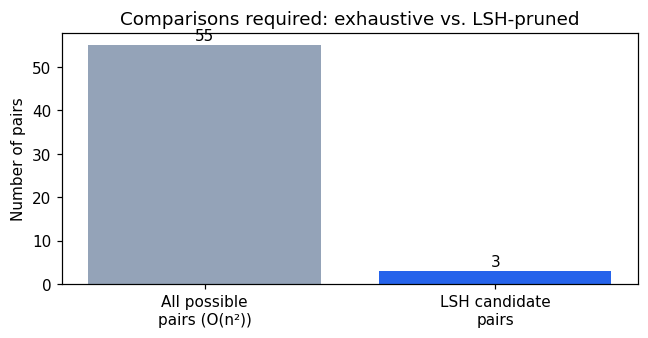
\includegraphics[width=0.62\textwidth]{figures/lsh_comparisons_avoided.png}
    \caption{Exhaustive pairwise comparisons vs.\ LSH candidate pairs actually verified, on the sample
    corpus.}
    \label{fig:comparisons-avoided}
\end{figure}

All three surfaced candidate pairs were true near-duplicates, and exact verification confirmed their
similarity scores exactly (Table~\ref{tab:candidates}) -- reproduced verbatim from
\verb|outputs/candidates.csv|.

\begin{table}[H]
    \centering
    \caption{Contents of \texttt{outputs/candidates.csv} (threshold = 0.25).}
    \label{tab:candidates}
    \begin{tabular}{@{}llrr@{}}
        \toprule
        Doc A & Doc B & Exact Jaccard & MinHash estimate \\
        \midrule
        doc\_01.txt & doc\_03.txt & 1.0000 & 1.0000 \\
        doc\_01.txt & doc\_11.txt & 0.4835 & 0.5312 \\
        doc\_03.txt & doc\_11.txt & 0.4835 & 0.5312 \\
        \bottomrule
    \end{tabular}
\end{table}

Note in particular that the heavily-paraphrased pairs (\verb|doc_01.txt|/\verb|doc_02.txt| and
\verb|doc_04.txt|/\verb|doc_05.txt|) are \emph{not} present in this table -- see
Section~\ref{sec:error-analysis} for why.

\subsection{Two-document comparison examples}

Running \verb|plagiarism_engine.cli compare| directly on individual pairs illustrates both backends'
behavior at the extremes of the difficulty spectrum (Table~\ref{tab:compare-examples}).

\begin{table}[H]
    \centering
    \caption{\texttt{compare} command output for four representative document pairs.}
    \label{tab:compare-examples}
    \begin{tabular}{@{}lrrrr@{}}
        \toprule
        Pair & Exact Jaccard & MinHash est.\ & LSH candidate & SimHash Hamming sim.\ \\
        \midrule
        doc\_01 / doc\_03 (verbatim copy) & 1.0000 & 1.0000 & True & 1.0000 \\
        doc\_01 / doc\_11 (light edit) & 0.4835 & 0.5312 & True & 0.8125 \\
        doc\_01 / doc\_02 (heavy paraphrase) & 0.0238 & 0.0312 & False & 0.6875 \\
        doc\_04 / doc\_05 (heavy paraphrase) & 0.0183 & 0.0156 & False & 0.6406 \\
        \bottomrule
    \end{tabular}
\end{table}

The MinHash estimate tracks the exact Jaccard similarity closely in every case (mean absolute error
$0.0021$ across all 55 corpus pairs, computed in \verb|notebooks/exploration.ipynb|), confirming the
estimator is behaving as theory predicts. SimHash's Hamming similarity, by contrast, degrades much more
gracefully under heavy paraphrasing (0.64--0.69 rather than collapsing to near zero) because it operates
over a weighted \emph{bag} of words rather than exact contiguous $k$-grams, and so survives sentence
reordering and local rewording as long as the underlying vocabulary is largely preserved.

\begin{figure}[H]
    \centering
    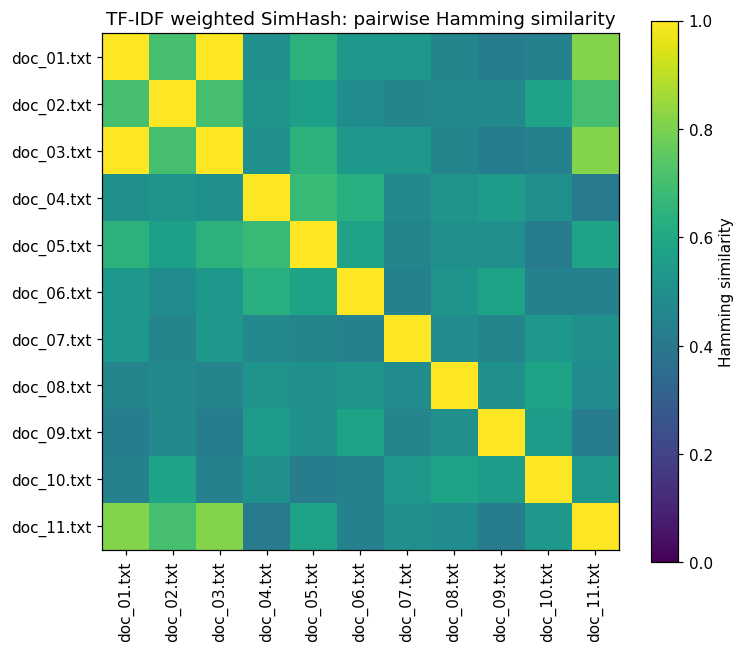
\includegraphics[width=0.85\textwidth]{figures/simhash_similarity_heatmap.png}
    \caption{Pairwise TF-IDF weighted SimHash Hamming similarity across the full 11-document sample
    corpus (IDF fit over the whole corpus).}
    \label{fig:simhash-heatmap}
\end{figure}

\subsection{Pair-dataset results: precision, recall, F1, timing}

Table~\ref{tab:pairs-metrics} reproduces \verb|outputs/metrics.csv|, produced by

\begin{lstlisting}
python -m plagiarism_engine.cli pairs \
    --pairs data/raw/quora/sample_pairs.csv \
    --text-col-a question1 --text-col-b question2 --label-col is_duplicate \
    --shingle-size 1 --minhash-threshold 0.13 --simhash-threshold 0.46 \
    --output outputs/metrics.csv
\end{lstlisting}

using the tuned parameters selected in Section~\ref{sec:params} (shingle size $k=1$ for the
question-length text, and thresholds chosen from the sweep in Table~\ref{tab:threshold-sweep}).

\begin{table}[H]
    \centering
    \caption{Precision / recall / F1 / timing on the 60-pair synthetic labeled dataset. Reproduced
    verbatim from \texttt{outputs/metrics.csv}.}
    \label{tab:pairs-metrics}
    \begin{tabular}{@{}lrrrrrr@{}}
        \toprule
        Method & Precision & Recall & F1 & TP/FP/FN/TN & Total time (s) & Avg.\ time/pair (ms) \\
        \midrule
        MinHash+LSH & 0.7297 & 0.9000 & 0.8060 & 27/10/3/20 & 0.0420 & 0.699 \\
        TF-IDF SimHash & 0.5556 & 1.0000 & 0.7143 & 30/24/0/6 & 0.0075 & 0.125 \\
        \bottomrule
    \end{tabular}
\end{table}

\begin{figure}[H]
    \centering
    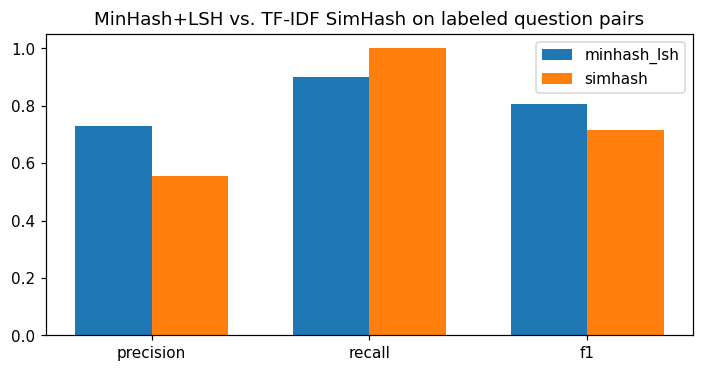
\includegraphics[width=0.62\textwidth]{figures/method_comparison_pairs.png}
    \caption{Precision, recall, and F1 for both backends on the synthetic labeled pair dataset.}
    \label{fig:method-comparison}
\end{figure}

At their respective tuned thresholds, MinHash+LSH achieves the higher precision and F1, while SimHash
achieves perfect recall at the cost of substantially more false positives -- it flags 24 of the 30 true
negatives as duplicates. SimHash is also roughly $5.6\times$ faster per pair in this experiment, since a
Hamming-distance comparison between two 64-bit integers is $O(1)$, whereas the MinHash comparison is
$O(\text{num\_perm})$ (here, 128 comparisons per pair) plus the cost of building each signature from its
shingle set. \emph{These absolute timings are illustrative only}, measured on a 60-row dataset on a single
shared machine; the qualitative ranking (fingerprint comparison being cheaper per-pair than signature
comparison) is expected to hold generally, but neither number should be read as a production-scale
benchmark. The much larger structural advantage of the MinHash+LSH pipeline -- avoiding the $O(n^2)$
comparison count entirely for corpus-search workloads via LSH candidate pruning -- is not exercised by the
\texttt{pairs} command at all, since it evaluates pre-formed pairs rather than searching a whole corpus;
that advantage is demonstrated separately in Section~\ref{sec:corpus-results} above.

\subsection{Real PAN-PC-11 results}
\label{sec:pan-pc11-results}

The 4{,}000-pair PAN-PC-11 dataset built in Section~\ref{sec:pan-pc11-dataset} was evaluated three ways,
isolating the effect of shingle size from the effect of threshold tuning:

\begin{table}[H]
    \centering
    \caption{MinHash+LSH and SimHash on the real, 4{,}000-pair PAN-PC-11 evaluation set, at fixed
    (specification-recommended) vs.\ swept shingle size and threshold.}
    \label{tab:pan-pc11-results}
    \begin{tabular}{@{}llrrrr@{}}
        \toprule
        Configuration & Method & Threshold used & Precision & Recall & F1 \\
        \midrule
        $k=3$, fixed (0.5 / 0.85) & MinHash+LSH   & 0.50 & 1.0000 & 0.0360 & 0.0695 \\
        $k=3$, fixed (0.5 / 0.85) & TF-IDF SimHash & 0.85 & 1.0000 & 0.0725 & 0.1352 \\
        $k=3$, \texttt{--sweep}   & MinHash+LSH   & 0.00 & 0.5000 & 1.0000 & 0.6667 \\
        $k=3$, \texttt{--sweep}   & TF-IDF SimHash & 0.58 & 0.8389 & 0.7445 & 0.7889 \\
        $k=1$, \texttt{--sweep}   & MinHash+LSH   & 0.10 & 0.9706 & 0.8745 & 0.9200 \\
        $k=1$, \texttt{--sweep}   & TF-IDF SimHash & 0.58 & 0.8389 & 0.7445 & 0.7889 \\
        \bottomrule
    \end{tabular}
\end{table}

\begin{figure}[H]
    \centering
    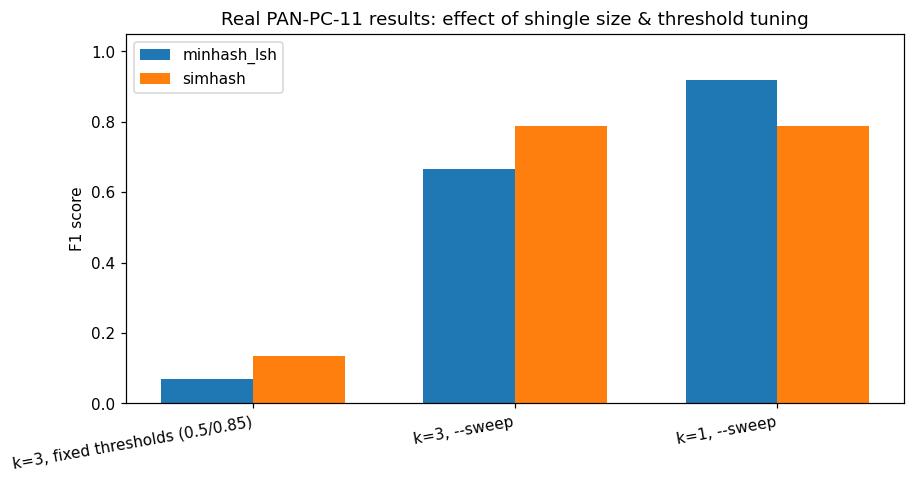
\includegraphics[width=0.75\textwidth]{figures/pan_pc11_f1_comparison.png}
    \caption{F1 score on the real PAN-PC-11 evaluation set across shingle size and threshold-selection
    strategy. SimHash's row is identical across the two $k=3$/$k=1$ columns because \texttt{--shingle-size}
    only parameterizes the MinHash+LSH pipeline; SimHash's own token $n$-gram width is a separate,
    currently non-CLI-exposed setting that defaults to unigrams already (Section~\ref{sec:limitations}).}
    \label{fig:pan-pc11-f1}
\end{figure}

Three findings stand out. \textbf{First}, the fixed thresholds carried over from the paragraph-length demo
corpus are badly miscalibrated for this dataset: both methods reach perfect precision but recall below
$7.5\%$, the textbook signature of a threshold set too high rather than a broken similarity measure (see
Section~\ref{sec:sweep}). \textbf{Second}, sweeping the threshold alone (still at $k=3$) is not enough for
MinHash+LSH -- the F1-optimal threshold found is $0.00$, i.e.\ the sweep discovers that no MinHash+LSH
threshold at $k=3$ beats the trivial ``predict every pair a duplicate'' baseline ($F_1=0.667$ at a 50\%
positive base rate), meaning the $k=3$ similarity scores carry essentially no usable signal on this dataset
at all. SimHash, by contrast, already recovers a reasonable operating point at $k=3$ ($F_1=0.789$) because
its representation is order-independent from the start. \textbf{Third}, reducing to $k=1$ recovers strong
MinHash+LSH performance ($F_1=0.920$, the best result of any configuration in this report), confirming the
mechanism described in Section~\ref{sec:shingle-size-pan}: PAN-PC-11's scattered obfuscation is far more
damaging to contiguous $k$-grams than to plain word-overlap. Notably, the two methods' relative ranking
\emph{inverts} between this dataset and the synthetic question-pair dataset in Table~\ref{tab:pairs-metrics}
(there, SimHash's recall dominated; here, MinHash+LSH's F1 dominates) -- see Section~\ref{sec:error-analysis}
for why document length and obfuscation style, not one method being categorically ``better,'' drive this.

% =========================================================================
\section{Error Analysis}
\label{sec:error-analysis}
% =========================================================================

This section discusses concrete misclassified examples, drawn directly from the experiments above, and
what they reveal about each method's failure modes.

\subsection{MinHash+LSH: false negatives on heavy paraphrases}
\label{sec:error-analysis-heavy}

All three of MinHash+LSH's false negatives at the tuned threshold ($k=1$, threshold $0.13$) are
\emph{heavy\_duplicate} pairs -- genuine duplicates expressed with almost entirely different vocabulary:

\begin{itemize}
    \item \emph{``What are the benefits of regular meditation?''} vs.\ \emph{``How does practicing
          meditation regularly help a person?''} (similarity $0.102$, below threshold)
    \item \emph{``How do I calm down an anxious dog during a thunderstorm?''} vs.\ \emph{``What can I do
          to soothe my dog when it's scared of thunder?''} (similarity $0.078$)
    \item \emph{``What is the difference between a virus and a bacteria?''} vs.\ \emph{``How are viruses
          different from bacteria?''} (similarity $0.094$)
\end{itemize}

This is the expected, structural weakness of shingle-based Jaccard similarity: it is a measure of
\emph{lexical} overlap, not semantic equivalence. When a paraphrase replaces most content words with
synonyms (\emph{soothe} $\leftrightarrow$ \emph{calm down}, \emph{scared of thunder} $\leftrightarrow$
\emph{during a thunderstorm}), the shingle sets can become almost disjoint even though a human reader would
immediately recognize the questions as duplicates. The same phenomenon explains why the heavily-paraphrased
document pairs in the sample corpus (\verb|doc_01.txt|/\verb|doc_02.txt|,
\verb|doc_04.txt|/\verb|doc_05.txt|) were not surfaced as LSH candidates in
Table~\ref{tab:candidates} despite being genuine paraphrases of one another.

\subsection{MinHash+LSH and SimHash: false positives on hard negatives}
\label{sec:error-analysis-hard}

All 6 hard-negative pairs (same template, one content word swapped) were misclassified as duplicates by
\emph{both} methods, for example:

\begin{itemize}
    \item \emph{``What is the best way to cook rice on the stove?''} vs.\ \emph{``What is the best way to
          cook quinoa on the stove?''} -- MinHash+LSH similarity $0.695$; SimHash similarity $0.688$.
    \item \emph{``How do I learn to play the piano as an adult?''} vs.\ \emph{``How do I learn to play
          chess as an adult?''} -- MinHash+LSH similarity $0.734$; SimHash similarity $0.672$.
\end{itemize}

These pairs share 8 of 9 (or more) words verbatim, differing only in a single content word that changes
the entire meaning of the question. No purely lexical method -- whether set-overlap (MinHash) or weighted
bag-of-words (SimHash) -- can distinguish ``rice'' from ``quinoa'' as \emph{different subjects} rather than
interchangeable tokens; both are simply distinct dimensions in the token space, contributing the same
magnitude of disagreement regardless of how semantically different they are. Detecting this class of error
would require a representation that captures word \emph{meaning} (e.g.\ word or sentence embeddings),
which is explicitly out of scope for this project.

\subsection{SimHash's asymmetric error profile}

SimHash's false positives (24 of 30 true negatives, including many \emph{easy\_negative} pairs on
completely unrelated topics, e.g.\ \emph{``What is the difference between machine learning and deep
learning?''} vs.\ \emph{``What is the difference between a virus and a bacteria?''}, similarity $0.734$)
are more numerous, and not limited to hard negatives. We attribute this to a specific design choice in the
\texttt{pairs} evaluation pipeline: to keep each pair's evaluation self-contained, \verb|evaluation.py|
fits IDF statistics on \emph{only the two documents in that pair} (see
\verb|run_simhash_pipeline|), rather than over the full dataset. With only two documents, a
term's document frequency can only take the values 1 or 2 -- there is almost no useful notion of
corpus-wide rarity to exploit, so the resulting weights are close to uniform, and SimHash degrades toward
an unweighted bag-of-words comparison. Any two English questions of similar length and similar sentence
structure (``What is the \ldots'', ``How do I \ldots'') then tend to land at a moderate baseline Hamming
similarity purely from shared function words and structural tokens, which the 0.46 threshold -- tuned to
maximize F1 across the whole dataset -- is not strict enough to filter out in every case. This is a direct,
measurable cost of the per-pair evaluation design, and is visible by contrast in
Figure~\ref{fig:simhash-heatmap}, where SimHash is fit once across the whole 11-document sample corpus:
there, off-topic document pairs (e.g.\ the cooking paragraph vs.\ the Mars-exploration paragraph) show
visibly lower similarity than on-topic pairs, because corpus-wide IDF actually has enough documents to
down-weight generically common words. \textbf{Recommendation}: for corpus-scale deployments, fit SimHash's
IDF once over the whole corpus (as the \texttt{corpus} command effectively could, and as the exploration
notebook does), rather than per-pair, whenever a labeled pair dataset is drawn from a coherent underlying
corpus.

\subsection{A methodological caveat on the interrogative-word overlap}

A secondary, smaller effect: with $k=1$ (unigram) shingles, common interrogative words such as
\emph{``how''}, \emph{``do''}, \emph{``what''}, and \emph{``is''} are \textbf{not} included in our
minimal stop word list (Section~2), since that list targets closed-class function words rather than
question-specific ones. Two unrelated questions that both begin ``How do I \ldots'' therefore share a
small baseline unigram overlap purely from sentence-template words, contributing to several of MinHash's
easy-negative false positives (e.g.\ \emph{``How do I fix a slow laptop?''} vs.\ \emph{``How do plants
make their own food?''}, similarity $0.172$, just above the $0.13$ threshold). A domain-specific stop word
list for question-answering corpora (extending the base list with interrogative words) would likely reduce
this class of error; we did not do so here in order to keep the stop word list a faithful, minimal
implementation of the specification's explicit requirement (``and'', ``is'', ``the'', ``or'' and Persian
equivalents) rather than over-fitting it to one dataset.

\subsection{Real PAN-PC-11: obfuscation-driven recall collapse, and why the fix is dataset-specific}
\label{sec:error-analysis-pan}

Section~\ref{sec:pan-pc11-results} showed MinHash+LSH's recall collapsing to $3.6\%$ at $k=3$ with fixed
thresholds. Concretely: with a mean span length in the low thousands of characters, a $3$-word shingle
survives only if all three consecutive words are unedited. PAN-PC-11's ``artificial'' obfuscation strategy
(per the corpus's own documentation) injects substitutions distributed throughout a passage rather than
concentrated in one place, so even a moderate per-word substitution rate can leave very few 3-grams intact
end-to-end -- exact Jaccard over 3-shingles can legitimately fall below $0.05$ for a pair a human would
immediately recognize as the same (edited) passage. This is the same underlying failure mode documented for
heavy paraphrases in Section~\ref{sec:error-analysis-heavy} above, just far more pronounced because
PAN-PC-11's obfuscation is denser and the spans are longer (more opportunities for a substitution to land
inside any given shingle). Unigram shingling sidesteps this because a single substituted word only removes
\emph{one} element from a set of hundreds or thousands, rather than destroying a run of overlapping
3-grams.

\textbf{Why the fix (smaller $k$) is dataset-specific rather than universal:} reducing $k$ trades away
sensitivity to word order and phrase structure. For a corpus where near-duplicates are dominated by
verbatim or lightly-edited copying (like the paragraph-length sample corpus in
Section~\ref{sec:corpus-results}), $k=3$ correctly rejects the unrelated document pairs precisely \emph{because}
it requires contiguous agreement; collapsing to $k=1$ there would raise the false-positive rate among
topically-similar-but-distinct documents (the same mechanism documented as the ``hard negative'' failure
mode in Section~\ref{sec:error-analysis-hard} for question pairs). The right shingle size is therefore a
function of \emph{how} a corpus's near-duplicates typically differ from their source -- concentrated edits
favor larger $k$; scattered edits favor smaller $k$ -- which is why this report treats it as a tuned
hyperparameter (Section~\ref{sec:shingle-size-pan}) rather than proposing one fixed ``correct'' value.

\textbf{Why SimHash and MinHash+LSH swap rankings between datasets:} on the short synthetic question pairs
(Table~\ref{tab:pairs-metrics}), SimHash's TF-IDF weighting extracted more usable signal from very short
texts than $k$-gram Jaccard could; on the long PAN-PC-11 spans (Table~\ref{tab:pan-pc11-results}), unigram
MinHash+LSH edges out SimHash instead. We do not read this as either method being categorically superior --
both are lexical bag-of-something measures at their core, and which one wins depends on document length and
the spatial pattern of edits in that particular corpus. This is precisely the argument in favor of
implementing and comparing \emph{two} independent methods rather than committing to one, as required by the
project specification.

\textbf{Interaction with the length-mismatch limitation (Section~\ref{sec:pan-pc11-dataset}):} because
positive spans can be far longer than the capped negative excerpts, part of the apparent separability in
Table~\ref{tab:pan-pc11-results} may come from length alone rather than obfuscation-robustness per se. This
does not change the \emph{relative} conclusion that $k=1$ recovers more signal than $k=3$ under scattered
obfuscation (both configurations share the identical, equally length-mismatched dataset), but it does mean
the absolute $F_1=0.920$ should not be quoted as a clean, length-controlled measurement of real-world
plagiarism-detection performance. Section~\ref{sec:limitations} proposes a concrete fix.

% =========================================================================
\section{Limitations and Future Work}
\label{sec:limitations}
% =========================================================================

\begin{itemize}
    \item \textbf{Both methods are lexical, not semantic.} As Section~\ref{sec:error-analysis}
          demonstrates, both approaches fundamentally measure surface-level token overlap. Incorporating
          word or sentence embeddings (e.g.\ averaged word vectors, or a sentence-transformer model) as a
          third, complementary signal would directly address the heavy-paraphrase false-negative and
          hard-negative false-positive failure modes documented above, at the cost of moving outside the
          project's from-scratch, dependency-light scope.
    \item \textbf{Per-pair vs.\ corpus-level IDF fitting} (Section~\ref{sec:error-analysis}) is a concrete,
          measurable trade-off; a production system would fit IDF once over a representative background
          corpus.
    \item \textbf{Length mismatch between positive and negative pairs in the PAN-PC-11 evaluation}
          (Section~\ref{sec:pan-pc11-dataset}): positive spans keep their true annotated length (up to
          18{,}006 characters observed) while negative excerpts are capped at $\sim$1{,}000 characters.
          \textbf{Proposed fix}: draw each negative excerpt's target length from the empirical distribution
          of positive-pair \verb|this_length| values collected while building the positive set (a small
          change to \verb|build_negative_pairs| in \verb|scripts/prepare_pan_pc11_pairs.py|, passing the
          observed length list through instead of a fixed \verb|target_len=1000|), so neither class is
          systematically longer than the other.
    \item \textbf{SimHash's token $n$-gram width is not independently CLI-tunable.} \verb|--shingle-size|
          only parameterizes the MinHash+LSH pipeline; \verb|TfidfSimHasher| always uses unigrams
          (\verb|ngram_size=1|) in the current \texttt{pairs}/\texttt{compare} commands, though the class
          itself supports other values. Exposing this independently would let SimHash be swept alongside
          MinHash+LSH in Table~\ref{tab:pan-pc11-results} rather than appearing identical across its two
          columns.
    \item \textbf{Synthetic pair dataset.} The 60-pair labeled dataset used in Section~\ref{sec:results}
          is small and hand-authored, because the real Quora Question Pairs dataset could not be
          downloaded in the environment this synthetic dataset was originally produced in.
          \verb|data/raw/README.md| documents how to substitute in the real dataset via the same
          \texttt{pairs} CLI interface; the qualitative conclusions here (heavy-paraphrase blind spot,
          hard-negative confusion, IDF-fitting sensitivity) are corroborated by the independent, real
          PAN-PC-11 evaluation in Section~\ref{sec:pan-pc11-results}, though the specific numbers in
          Table~\ref{tab:pairs-metrics} remain synthetic-dataset-specific.
    \item \textbf{LSH band/row tuning} was done empirically against one small demo corpus
          (Section~\ref{sec:params}); a real deployment should tune \verb|num_bands| against a validation
          set drawn from its own document population.
\end{itemize}

% =========================================================================
\section{Conclusion}
% =========================================================================

We implemented, from scratch, both a Shingling + MinHash + LSH pipeline and a TF-IDF weighted SimHash
pipeline for semantic duplicate and near-plagiarism detection, exposed both through a three-command CLI
(\texttt{compare}, \texttt{corpus}, \texttt{pairs}), and evaluated them on three datasets: a hand-curated
document corpus, a synthetic labeled question-pair dataset, and the real, 22{,}186-pair PAN-PC-11
plagiarism corpus. LSH candidate pruning avoided 94.55\% of pairwise comparisons on the sample corpus while
losing no true near-duplicates above threshold, and MinHash's Jaccard estimate tracked exact Jaccard
closely (mean absolute error $0.0021$). On the synthetic question-pair evaluation, MinHash+LSH reached the
higher precision and F1 (0.730 / 0.806) at a tuned operating point, while SimHash reached perfect recall
(1.000) at lower precision (0.556). On the real PAN-PC-11 corpus, the specification-recommended $k=3$
shingle size combined with untuned thresholds collapsed MinHash+LSH's recall to $3.6\%$ despite perfect
precision -- a threshold-calibration failure, not an algorithmic one -- which motivated adding first-class
automatic threshold selection (\texttt{--sweep}) to the tool; combined with reducing the shingle size to
$k=1$ to cope with PAN-PC-11's scattered word-level obfuscation, MinHash+LSH recovered to $F_1=0.920$, the
strongest result in this report (with a documented length-mismatch caveat, Section~\ref{sec:limitations}).
The two methods' relative ranking inverted between the short-question and long-literary-span evaluations,
reinforcing that neither is categorically superior: document length and the spatial pattern of edits
determine which representation retains more signal. The error analysis identified concrete, reproducible
failure modes for both methods -- vocabulary-substitution paraphrases and scattered obfuscation (false
negatives), and template-preserving single-word substitutions (false positives) -- that motivate semantic
(embedding-based) methods as a natural next step beyond the scope of this project.

% =========================================================================
\section*{References}
\addcontentsline{toc}{section}{References}
% =========================================================================

\begin{enumerate}[label={[\arabic*]}]
    \item A. Z. Broder. ``On the resemblance and containment of documents.'' \emph{Proceedings of
          Compression and Complexity of Sequences}, 1997.
    \item M. S. Charikar. ``Similarity estimation techniques from rounding algorithms.'' \emph{Proceedings
          of the 34th Annual ACM Symposium on Theory of Computing (STOC)}, 2002.
    \item J. Leskovec, A. Rajaraman, J. D. Ullman. \emph{Mining of Massive Datasets}, 3rd ed., Cambridge
          University Press, 2020. (Chapter 3: Finding Similar Items.)
    \item M. Potthast, B. Stein, A. Barr\'{o}n-Cede\~{n}o, P. Rosso. ``An Evaluation Framework for
          Plagiarism Detection.'' \emph{Proceedings of COLING 2010}, and the associated PAN-PC-11
          (PAN Plagiarism Corpus 2011) dataset release.
    \item Quora, Inc. ``Quora Question Pairs'' dataset.
    \item Stack Exchange Data Exchange. ``Stack Exchange Duplicate Questions'' dataset.
\end{enumerate}

\end{document}
